%Vodní toky jsou významnou složkou krajiny. Potůčky, potoky, řeky odvádějí vodu z krajiny zpět do oceánů. Vodní toky jsou významným tvůrcem krajiny. Unášejí velké množství sedimentů a rozpuštěných látek. Podílejí se na denudaci
\section{Fluviální systém}
Vodní toky jsou jen jednou z částí \emph{fluviálního systému} (Obr. \ref{fig:fluvsystem}). Fluviální systém propojuje svahy, údolní nivy, říční síť a další části do jednoho celku, prostřednictvím kterého dochází k pohybu vody a sedimentů. Jelikož se jedná o otevřený systém, dochází k výměně energie a látek (vody, sedimentů) s jeho okolím. 

Hlavními vstupy do fluviálního systému jsou voda a sedimenty. Dalším vstupem může být například organický materiál (dřevo). Převážná část energie pohánějící celý systém pochází z atmosférických procesů (výpar, kondenzace, srážky). V podstatě zvyšují potenciální energii vody (dostává se do vyšších poloh). Díky gravitaci se pak voda dává do pohybu, tedy potenciální energie se mění na kinetickou. Část energie je pak vynaložena na transport sedimentů.

Výstup z fluviálního systému je zpravidla v místě ústí vodního toku do sedimentační pánve (jezero, moře, oceán...). 

Ve fluviálním systému dochází ale i k ukládání materiálu. Voda je v jezerech, vodních nádržích. Sedimenty jsou uložené v korytě, jezerech, nivách.

% TODO: \usepackage{graphicx} required
\begin{figure*}
	\centering
	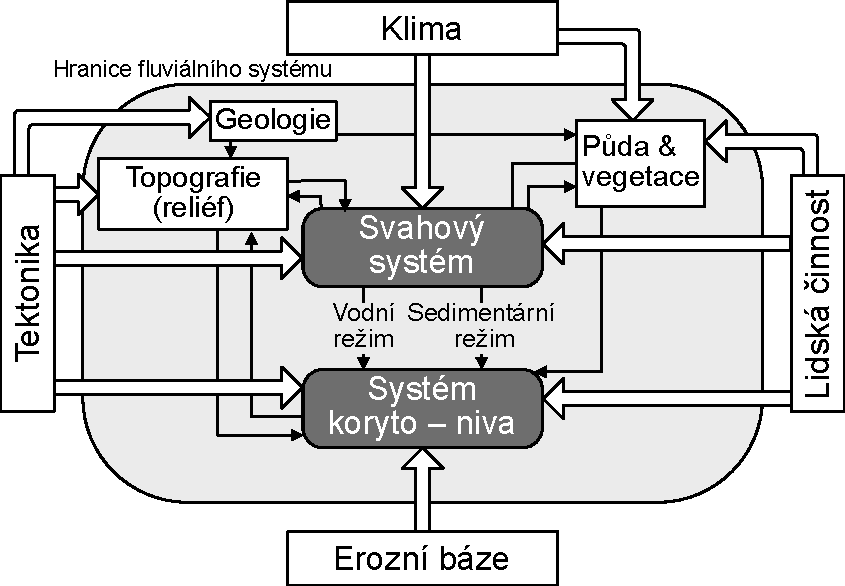
\includegraphics[width=0.9\linewidth]{obrazky/fluvial/fluv_system}
	\caption{Zjednodušené schéma fluviálního systému (upraveno podle \textcite{charltonFundamentalsFluvialGeomorphology2007}.)}
	\label{fig:fluvsystem}
\end{figure*}

\section{Proudění vody v korytech}
Proudění je neuspořádaný pohyb částic tekutiny (vody) převážně jedním směrem. Díky gravitaci teče voda v korytech shora dolů. Tomuto pohybu brání tření na rozhraní voda-koryto, ale i vnitřní tření vlastní vody. 

Proudění může být \emph{ustálené} neboli stacionární (\textit{steady flow}). Při tomto typu proudění se částice pohybují jedním směrem a se stále stejnou rychlostí -- průtok se nemění.  Opakem je \emph{neustálené proudění} neboli nestacionární (\textit{unsteady flow}), kdy se rychlost v závislosti na čase mění.

\emph{Rovnoměrné (uniformní) proudění} (\textit{uniform flow}) je ustálené proudění, při kterém jsou konstantní další parametry toku (např. průtočná plocha). Při \emph{nerovnoměrném proudění} (\textit{non-uniform flow}) se průtok nemění, ale mění se rychlost proudění, průtočná plocha a další parametry. 

\subsection{Charakter proudění v korytech}
\emph{Laminární proudění} je takové proudění, kdy se kapalina pohybuje ve vrstvách -- laminách, které navzájem kloužou po sobě (Obr. \ref{fig:laminarturbul}). Laminárním prouděním jsou typické vysoce viskózní kapaliny. Jelikož voda má malou viskozitu, laminární proudění se projevuje jen při nízkých rychlostech.
\emph{Turbulentní proudění} je chaotické a všesměrné (Obr. \ref{fig:laminarturbul}). Pohyb je realizován po i proti proudu, do stran, nahoru či dolů. 

% TODO: \usepackage{graphicx} required
\begin{figure}[h]
	\centering
	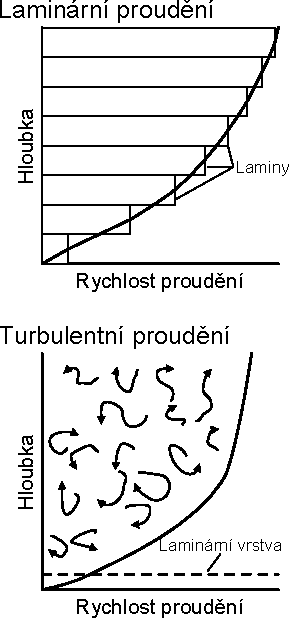
\includegraphics[width=1\linewidth]{obrazky/fluvial/laminar_turbul}
	\caption{Laminární a turbulentní proudění.}
	\label{fig:laminarturbul}
\end{figure}


\emph{Reynoldsovo číslo} vyjadřuje, zda proudění bude laminární nebo turbulentní. Jedná se o bezrozměrné číslo, které je dáno poměrem inertních sil a viskózních sil.

\begin{equation}\label{key}
	Re = \frac{\text{Inerční síly}}{\text{viskózní síly}} = \frac{vR}{\nu_{s}}
\end{equation}

\begin{eqexpl}
	\item{$Re$}Reyonoldsovo číslo (bezrozměrné)
	\item{$v$}Rychlost proudění [\si{\metre\per\second}]
	\item{$R$} je hydraulický poloměr [\si{\metre}]
	\item{$\nu_{s}$} je kinematická viskozita [\si{\metre\squared\per\second}]
\end{eqexpl}

Laminární proudění je do hodnoty $Re$ < $500$ při hodnotách $Re$ = $500$ -- $1000$ má proudění přechodný charakter. Turbulentní proudění má hodnoty $Re$ > $2000$.

Na základě \emph{Froudeho čísla ($Fr$)} rozdělujeme proudění na \emph{bystřinné} a \emph{říční}. Pokud je $Fr >1$ jedná se proudění \emph{bystřinné} neboli \emph{nadkritické} (\textit{supercritical flow}). V případě $Fr <1$ jde o \emph{říční (podkritické) proudění} (\textit{subcritical flow}). $Fr = 1$ značí \emph{kritické} proudění. Froudeho číslo je závislé na rychlosti a hloubce proudění:

\begin{equation}
	Fr=\frac{v}{\sqrt{gd}}
\end{equation}

\begin{eqexpl}
	\item{$Fr$} Freudeho číslo (bezrozměrné)
	\item{$v$} Rychlost proudění [\si{\metre\per\second}]
	\item{$g$} tíhové zrychlení [\SI{9,81}{\metre\per\second\squared}]
	\item{$d$} hloubka proudění [\si{\metre}]
\end{eqexpl}

Ve většině případů je i v horských bystřinách říční proudění. Bystřinné (nadkritické) proudění se vyskytuje jen lokálně. Nadkritické proudění je charakteristické menším turbulentním promícháváním vody, což způsobuje efektivnější a rychlejší tok korytem. Přechod mezi podkritickým a nadkritickým prouděním se na toku projevuje hydraulickým poklesem. V opačném případě, kdy dochází ke změně proudění ze nadkritického na podkritické, vzniká hydraulický skok. 
%\todo[inline]{obrázek hydraulický skok, pokles}

\subsection{Rychlost proudění, průtok}
Rychlost proudění vody v korytě je závislá na několika faktorech. Velký vliv má samozřejmě sklon koryta, kdy s zvětšujícím se sklonem roste i rychlost proudění. Jelikož je pohyb vody bržděn třením o dno a břehy, velice důležitým faktorem je \emph{relativní drsnost koryta}. Čím je menší relativní drsnost koryta (a tedy i výsledné tření), tím větší je rychlost proudění. Drsnost koryta je relativní vůči hloubce proudění (hloubce toku). Stejné koryto bude mít větší relativní drsnost při nízkých průtocích, než při vysokých. Představte si tok s minimálním průtokem, kde si voda hledá cestičky mezi valouny a to samé koryto za vyššího vodního stavu. Jednotlivé valouny, které při nízkém průtoku čněly nad vodu již na celkovou drsnost budou mít pramalý vliv. Při větší hloubce toku je totiž jen menší část ovlivněna třením na rozhraní voda-koryto. 

Z důvodu tření pozorujeme nejnižší rychlosti proudění u břehů a dna. Směrem k hladině rychlost proudění nelineárně narůstá. Maxima jsou kousek pod hladinou, jelikož na hladině dochází k tření vody o vzduch a také tam jsou přítomné víry, které proudění zpomalují.

\emph{Průtok} je definován jako objem vody, která proteče profilem vodního toku za jednotku času. Typicky je průtok vyjadřován v \si{\metre\cubed\per\second}. 
\begin{equation}
	Q=vA
\end{equation}
\begin{eqexpl}
	\item{$Q$} Průtok [\si{\metre\cubed\per\second}]
	\item{$v$} Rychlost proudění [\si{\metre\per\second}]
	\item{$A$} Průtočná plocha příčného profilu [\si{\metre\squared}]
\end{eqexpl}


\emph{Manningova rovnice} vyjadřuje vztah mezi rychlostí proudění v korytě a parametry koryta:
%Manningova rovnice
\begin{equation}\label{eq:manning}
	v = [R^{\nicefrac{2}{3}}S^{\nicefrac{1}{2}}]/n
\end{equation}

\begin{eqexpl}
	\item{$v$} rychlost proudění [\si{\metre\per\second}]
	\item{$R$} hydraulický poloměr [\si{\metre}]
	\item{$S$} sklon vodní hladiny[\si{\metre\per\metre}]
	\item{$n$} Manningův koeficient drsnosti [bezrozměrné]
\end{eqexpl}

% Please add the following required packages to your document preamble:
% \usepackage{booktabs}
\begin{table*}[]
	\begin{tabularx}{1\textwidth}{@{}Xlll@{}}
		\toprule
		Popis koryta                                                    & Minimum & Běžná hodnota & Maximum \\ \midrule
		Rovné koryto bez vegetace                                       & 0,025   & 0,030         & 0,033   \\
		Klikatící se koryto bez vegetace s občasnými tůněmi a mělčinami & 0,033   & 0,040         & 0,045   \\
		Klikatící se koryto s vegetací a kameny na dně                  & 0,035   & 0,045         & 0,050   \\
		Hodně zarostlé koryto s hlubokými tůněmi                        & 0,075   & 0,100         & 0,150   \\
		Horské toky, na dně štěrky, valouny, balvany občasně            & 0,030   & 0,040         & 0,050   \\
		Horské toky; valouny a velké balvany                            & 0,040   & 0,050         & 0,070  \\ \bottomrule
	\end{tabularx}
	\caption{Manningovy koeficienty drsnosti $n$ pro malé toky (šířka do \SI{30}{\metre}). Zdroj: \textcite{chowOpenchannelHydraulics1959}}
	\label{tab:manning}
\end{table*}

\section{Energie, práce a výkon vodních toků}
Pohyb vody, sedimentů, eroze. To vše zahrnuje vykonávání \emph{práce}, tedy působení síly na hmotu po určité dráze. \emph{Energie} z vyjadřuje schopnost hmoty konat práci. Hmota s větší potenciální energií má větší kapacitu konat práci. Jak práce, tak energie mají stejnou jednotku -- jouly [\si{\joule}]. \emph{Výkon} vyjadřuje množství vykonané práce za jednotku času, jednotka je joul za sekundu neboli watt [\si{\watt}].

Pohybem vody z vyšších nadmořských výšek do nižších se přeměňuje potenciální energie vody na kinetickou (Rov. \ref{eq:potkin}). Až $95 \%$ kinetické energie se třením přemění na teplo. Zbylá energie je transformována na samotný pohyb vodní masy, transport sedimentů, erozi dna a břehů. Malý zlomek energie je vynaložen na zvukové projevy. 

\begin{equation}\label{eq:potkin}
	\underset{\text{potenciální energie}}{mgh} \longrightarrow \underset{\text{kinetická energie}}{\frac{1}{2}m v^{2}}
\end{equation}

\begin{eqexpl}
	\item{$m$} hmotnost vody [\si{\kilo\gram}]
	\item{$g$} tíhové zrychlení [\si{\metre\per\second\squared}]
	\item{$h$} relativní výška [\si{\metre}]
	\item{$v$} je rychlost proudění[\si{\metre\per\second}]
\end{eqexpl}

Výkon vodních toků se měří ve wattech na jednotku délky [\si{\watt\per\metre}] a vyjadřuje kapacitu vodního toku transportovat sedimenty. \emph{Výkon vodního toku} ($\Omega$) je hlavně závislý na průtoku ($Q$) a jeho sklonu ($S$).

\begin{equation}\label{eq:vykontoku}
	\Omega = \rho g Q S
\end{equation}

\begin{eqexpl}
	\item{$\Omega$} výkon vodního toku [\si{\watt\per\metre}]
	\item{$\rho$} hustota vody [\si{\kilogram\per\metre\cubed}]
	\item{$Q$} průtok [\si{\metre\cubed\per\second}]
	\item{$S$} je sklon vodní hladiny[\si{\metre\per\metre}]
\end{eqexpl}

Často se používá \emph{specifický výkon toku}, který je definován jako podíl výkonu toku ($\Omega$) a šířky koryta ($W$): 

\begin{equation}\label{eq:spec_vykon}
	\omega = \frac{\Omega}{W}
\end{equation}

Odpadá tím vliv šířky toku na výkon a lze tak jednoduše srovnávat toky mezi sebou. 

Proudící voda v korytě působí na dno \emph{tečným neboli smykovým napětím} (\textit{shear stress}). Pro ustálené rovnoměrné proudění je toto tečné napětí definované takto:

\begin{equation}\label{eq:tecne}
	\tau_{b} = \rho g R S
\end{equation}

\begin{eqexpl}
	\item{$\tau_{b}$} tečné napětí [\si{\newton\per\metre\squared}]
	\item{$\rho$} hustota vody [\si{\kilogram\per\metre\cubed}]
	\item{$R$} Hydraulický poloměr [\si{\metre}]
	\item{$S$} je sklon vodní hladiny[\si{\metre\per\metre}]
\end{eqexpl}

Vztah mezi specifickým výkonem toku, tečným napětím ($\tau_{b}$) a průměrnou rychlostí v profilu ($\bar{v}$) je následovný:

\begin{equation}\label{eq:spec_vykon_tecne}
	\omega = \tau_{b} \bar{v}
\end{equation}

\section{Fluviální eroze}
Fluviální eroze je výsledkem celé řady procesů a faktorů, které se uplatňují. 

\subsection{Typy eroze}
Erozi dělíme podle směru jejího působení. Při \emph{lineární (hloubkové) erozi} řeka prohlubuje své koryto. Dochází k erozi říčního dna. Při \emph{boční (břehové, laterální) erozi} dochází k pohybu toku do stran a erozi břehů. Jako \emph{zpětnou erozi} označujeme zahlubování vodního toku, které postupuje proti proudu. Zahlubování začalo v nižších polohách a postupuje do vyšších nadmořských výšek. Stává se, že erozně aktivnější vodní tok (s intenzivní zpětnou erozí) se napojí na vodní tok z jiného povodí. Tomuto jevu se říká \emph{říční pirátství}. Intenzivněji erodující tok zvětší své povodí na úkor jiného toku. 

%\todo[inline]{eroze, říční pirátství}

\subsection{Erozní procesy}

\subsubsection{Eroze ve skalních korytech}
Jelikož dotace sedimentů do skalních koryt je často omezená, jejich podoba je dána hlavně erozní činností vody. 

Proudící voda může erozně působit několika způsoby. \emph{Koroze} je proces chemického rozpouštění na kontaktu proudící vody a podloží. Intenzita koroze je závislá na rozpustnosti podloží, nasycenosti vody, průtokem a rychlostí proudění. Koroze je důležitým procesem ve vápencových oblastech.

\emph{Abraze (koraze)} je proces mechanického působení a odnosu podloží koryta v důsledku působení transportovaných částic. Účinek abraze závisí na množství a velikosti částic, jejich kinetické energii a odolnosti podloží. Rychlost proudění má velký účinek, neboť kinetická energie se mění se čtvercem rychlosti. 

Samotná proudící voda působí mechanicky na podloží. Tlakem vodního proudu může vytrhávat zvětralé podloží (tzv. \emph{plucking}). Intenzivnější je \emph{kavitace}. Jedná se o erozní činnost explodujících vzduchových bublin ve vodě. Intenzivně se plucking projevuje u vodopádů a peřejí. Třetím typem je mechanického působení je \emph{evorze}, což je mechanické působení turbulentního proudění. Jeho působením vznikají evorzní prohlubně -- \emph{obří (evorzní) hrnce}.

\subsubsection{Eroze v aluviálních korytech}
Aluviální koryta jsou charakteristická hlavně boční erozí. Ta je mimo jiné závislá na charakteru materiálu tvořící břehy. Významný stabilizační efekt má vegetace.

Břehová eroze je výsledkem různých procesů. \textcite{charltonFundamentalsFluvialGeomorphology2007} je dělí do tří skupin:
\begin{enumerate}
	\item \emph{Přípravné oslabující procesy} jako je například namáčení a vysoušení materiálu. Procesy činící břeh náchylným k erozi.
	\item \emph{Fluviální procesy}, kdy jednotlivé částice a agregáty jsou uvedené do pohybu vodou.
	\item \emph{Svahové procesy} zahrnující kolaps břehů (sesuvy, břehové nátrže)
\end{enumerate}

Nízké ale strmé břehy tvořené kohezním materiálem často kolabují odkláněním (topplingem), kdy se blok překlopí do koryta (Obr. \ref{fig:bankerosion}a). Odlučná plocha je téměř vertikální. U vyšších ale méně strmých břehů vznikají v kohezních materiálech rotační sesuvy (Obr. \ref{fig:bankerosion}b). U břehů tvořených nekohezním materiálem převažují mělké sesuvy, nátrže a opad (Obr. \ref{fig:bankerosion}c). Často jsou břehy z nekohezního materiálu v podloží a jemného kohezního materiálu v nadloží. Erozí méně odolného nekohezního materiálu dochází k podemílání břehu a jeho následného kolapsu (Obr. \ref{fig:bankerosion}).

\begin{figure}
	\centering
	\includegraphics[width=1\linewidth]{obrazky/fluvial/bank_erosion}
	\caption{Procesy břehové eroze. Upraveno podle \textcite{charltonFundamentalsFluvialGeomorphology2007}}
	\label{fig:bankerosion}
\end{figure}

\subsection{Zdroje sedimentů}
Hlavním zdrojem sedimentů jsou svahy v povodí. Rychlost tvorby svahoviny, která se následně může dostávat do vodního toku je dána geologickou stavbou (litologií, geologickou strukturou), klimatickými podmínkami. Donášku sedimentů do toku ale i významně ovlivňuje i vegetace. 

V horských oblastech, kde svahy jsou strmé, se do koryta snadněji budou dostávat klasty větších rozměrů. V nížinných oblastech pak převažuje plošný splach jemných sedimentů. Významným zdrojem sedimentů jsou břehové nátrže. 

\section{Fluviální transport}
\subsection{Uvedení částic do pohybu}
Co je potřeba, aby vodní tok uvedl do pohybu jednotlivé klasty? Klast ležící na dně je pod vlivem sil, které jej chtějí uvést do pohybu a těch, které ho drží na místě. Pokud mobilizační síly převáží, klast se dá do pohybu (Obr \ref{fig:sily_klast}). Proti pohybu působí tíha částice (normálová komponenta) a také okolní klasty, které mohou danou částici blokovat. Proudící voda působí na klast silou, kterou lze rozdělit do dvou složek. \emph{Vztlaková síla} (\textit{lift}) působí směrem vzhůru. \emph{Tření} (\textit{drag force}) působí ve směru proudění. 

\begin{figure}
	\centering
	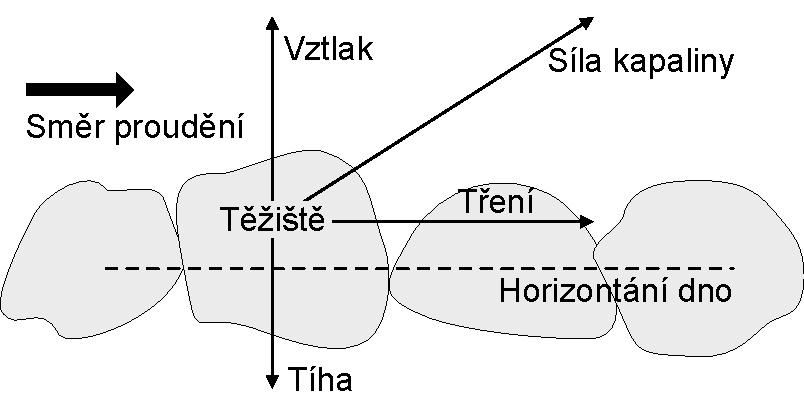
\includegraphics[width = 1\linewidth]{obrazky/fluvial/sily_klast}
	\caption{Síly působící na klast ve vodním toku \textcite{summerfieldGlobalGeomorphologyIntroduction1999}).}
	\label{fig:sily_klast}
\end{figure}

Kromě velikosti, hustoty, tvaru klastu hraje při jeho mobilizaci i to, jak je vystaven toku a také na rychlosti proudění nebo přesněji na kritickém tečném napětí. Tzv. Hjulstr\o{}mův diagram (Obr. \ref{fig:hjulstr}) znázorňuje při jakých rychlostech proudění se částice o dané velikosti začne pohybovat (je vodním tokem stržena), zůstává v pohybu a nebo sedimentuje. Tento diagram vznikl na základě laboratorních experimentů a ve volné přírodě jsou tyto vztahy složitější. Jak je z diagramu patrné, tak nejsnáz jsou erodované částice písku okolo \SIrange{0,1}{0,5}{\milli\metre}. Jílové částice jsou drženy pospolu kohezními silami, proto jsou nutné vyšší rychlosti proudění pro jejich uvedení do pohybu. 

\begin{figure*}
	\centering
	\includegraphics[width = 1\textwidth]{obrazky/fluvial/hjulstr}
	\caption{Hjulstr\o{}mův diagram znázorňující vztah mezi velikostí částice, rychlostí proudění a procesem (upraveno podle \textcite{hjulstromStudiesMorphologicalActivity1935})}
	\label{fig:hjulstr}
\end{figure*}

\begin{figure*}
	\centering
	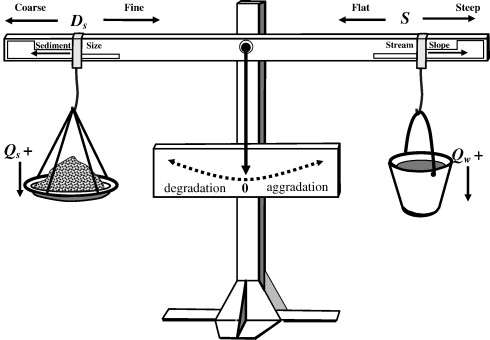
\includegraphics[width = 1\textwidth]{obrazky/fluvial/lanes_balance.jpg}
	\caption{Bilance mezi paramtry koryta, sedimenty, průtokem (převzato z \textcite{dustConceptualModelComplex2012})}
	\label{fig:vahy}
\end{figure*}

\subsection{Způsob fluviálního transportu}
Vodní toky transportují materiál ve dvou základních podobách -- rozpuštěný ve vodě a v pevném skupenství (klastický materiál) (Obr. \ref{fig:fluvsedtrans}). 

Klastický materiál transportovaný v suspenzi nazýváme \emph{plaveniny} (\textit{suspended load}).  V celém profilu vodního toku je koncentrace plavenin stejná, což je způsobené turbulentním prouděním. Plaveniny způsobují zakalení vody. V suspenzi je unášena většina ($70 \%$) z celosvětového množství unášeného materiálu řekami. V nížinných tocích plaveniny tvoří \SIrange{70}{95}{\percent} celkového objemu transportovaných sedimentů, bystřinné a štěrkonosné toky mají velké rozpětí (\SIrange{20}{90}{\percent}) závislé na dodávce hrubšího materiálu. 

\emph{Dnové splaveniny} (\textit{bed load}) jsou sedimenty, které se pohybují v kontaktu se dnem. Jednotlivé klasty se mohou sunout, válet se, nebo se pohybují poskakováním -- saltací. Dnové splaveniny mají velký geomorfologický efekt na koryto. S délkou transportu se zvětšuje opracování jednotlivých klastů (z ostrohranných se stávají zaoblené). Obecně také platí, že s délkou transportu a s délkou vodního toku se zmenšuje průměr částic.

\begin{figure}
	\centering
	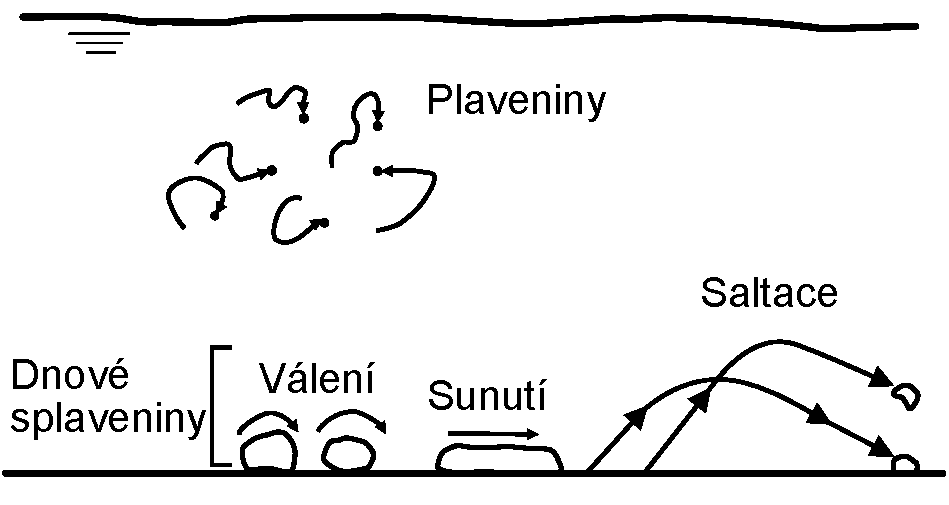
\includegraphics[width = 1\linewidth]{obrazky/fluvial/fluv_sed_trans}
	\caption{Fluviální transport klastických sedimentů. Rozpuštěné látky nejsou zobrazeny (upraveno podle \textcite{charltonFundamentalsFluvialGeomorphology2007}).}
	\label{fig:fluvsedtrans}
\end{figure}

\emph{Rozpuštěný materiál} (\textit{dissolved load}) je transportovaný v roztoku (např. ionty \ce{Ca^2+}, \ce{Mg^2+}, \ce{Na+}, \ce{SiO2}, \ce{HCO3-}, živiny na bázi fosforu, dusíku, rozpuštěné plyny. Globálně rozpuštěné látky odpovídají přibližně $20 \%$ celkové denudace. Koncentrace látek klesá s rostoucím průtokem. Morfologický efekt rozpuštěných látek na koryto je malý. 


\section{Říční koryto}
\subsection{Typy říčních koryt}
Rozlišují se tři typy říčních koryt. \emph{Aluviální} koryta jsou tvořena říčními sedimenty. \emph{Skalní} koryta jsou opakem aluviálních. Nachází se v nich minimální množství sedimentů a řeka je zahloubená do skalního podloží. Oba typy koryt ale nejsou ostře ohraničená, existuje tak \emph{přechodný typ}. 

\subsubsection{Skalní koryta}
Skalní koryta jsou  zařezaná do skalního podloží. To je činí poměrně stabilními. K bočním posunům koryta dochází v málo odolných horninách. Skalní koryta jsou zpravidla v horních částech toku, kde je větší sklon a řeka unáší hrubší materiál. Podélné profily skalních koryt jsou zpravidla nevyrovnané s velkým množstvím zálomů, tzv. knickpointů. Tyto zálomy jsou v místech, kde se dramaticky mění sklon koryta respektive je tam přítomen nějaký skok. Tento skok může být způsoben zlomem, mohou ho způsobovat sesuvy, které mohou zahradit údolní dno. 

\emph{Zakleslé meandry} (\enquote{intrenched meanders}) se nachází v místěch horizontálně uložených vrstev. Meandrující řeka se postupně zařezává do aluvia a postupem času se začne zakusovat i do skalního podloží. 

\subsubsection{Aluviální koryta}
Jak již bylo řečeno, aluviální koryta jsou tvořena vlastními říčními sedimenty. Tento typ koryt je velice různorodý, což je dáno variabilitou průtoku; množstvím, typem unášeného a ukládaného materiálu apod. Zároveň je tento typ koryt citlivý na změny v dodávkách sedimentů -- jejich množství a hrubosti, změny v průtoku, jelikož aluviální sedimenty snadno podléhají erozi. 

\subsubsection{Přechodná koryta}
Do kategorie spadající mezi aluviální a skalní koryta patři ty, které jsou lokálně ovlivněny skalním podložím případně jsou v aluviu odolném vůči erozi.

\subsection{Geometrický vzor toku}
Na rozdíl od skalních koryt mohou koryta v aluviu nabývat celé řady podob. Rozlišujeme několik základních vzorů. 

Podle sinuosity (poměr mezi délkou koryta k délce údolnice) rozlišujeme:

\begin{itemize}
	\item Přímá koryta
	\item Koryta se zákruty a meandry
	\item Divočící koryta
	\item Anastomózní koryta
\end{itemize}

\subsubsection{Přímé toky}
Čistě přímá aluviální koryta nejsou běžná. Zpravidla jsou vázaná na rovné úseky \enquote{V-údolí}, které jsou vázané na strukturní predispozice. Přímé toky v nížinách jsou zpravidla vždy výsledkem antropogenních úprav koryta. 

\subsubsection{Meandrující toky}
Meandrující toky jsou patrně nejrozšířenější formou. Jedná se o řeky, které se rozličně klikatí krajinou. Meandrující toky mají sinusoitu větší než $1,5$ \parencite{huggettFundamentalsGeomorphology2017}. Vlnová délka meandrů je přímo závislá na šířce koryta. Větší toky mají i větší vlnovou délku meandrů. Do tohoto vztahu vstupují ale i další faktory jako je například materiál aluvia. 

Meandry vznikají rozkmitáním proudnice a díky přítomnosti sekundárního tzv. heliakálního proudění. Toto proudění zvyšuje erozi na nárazovém \emph{výsepním} břehu a napomáhá sedimentaci na vnitřním \emph{jesepním} břehu. 

\begin{figure}
	\centering
	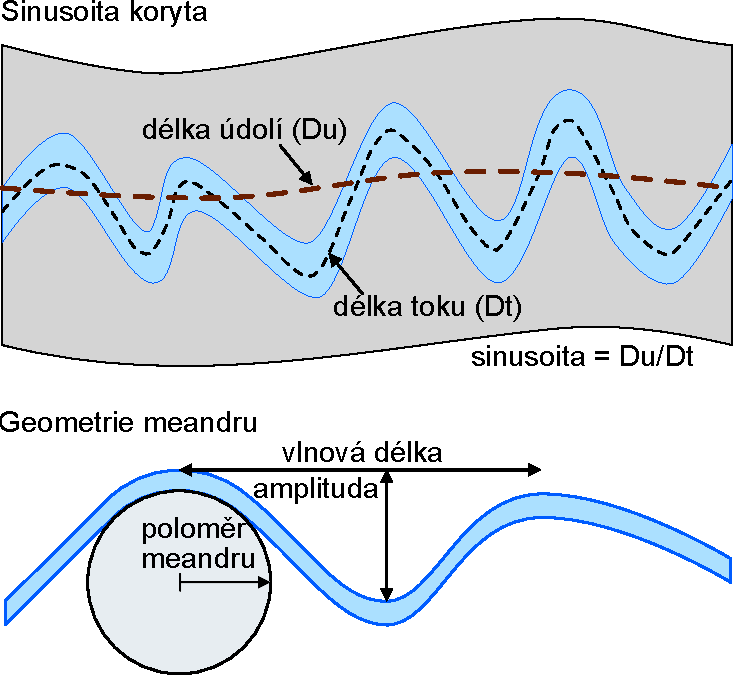
\includegraphics[width=1\linewidth]{obrazky/fluvial/mendry_sinusoita}
	\caption{Sinusoita koryta a geometrické parametry meandrů (upraveno podle \textcite{biermanKeyConceptsGeomorphology2014})}
	\label{fig:mendrysinusoita}
\end{figure}

\subsubsection{Divočící toky}
Vodní tok, který nese velké množství hrubého materiálu (štěrku) a má hodně rozkolísané průtoky vytváří tzv. divočící tok. Tento typ toků se nachází při vyústění horských toků do předpolí. Tok přetížený sedimenty je začne ukládat. Vznikají štěrkové lavice -- akumulace, které tok různě obtéká, větví se na nich. Typické je časté překládání koryta. Z důvodu velké dynamiky lavic se vegetace nestačí uchytit na štěrkových lavicích a stabilizovat je.

\begin{figure}[h]
	\centering
	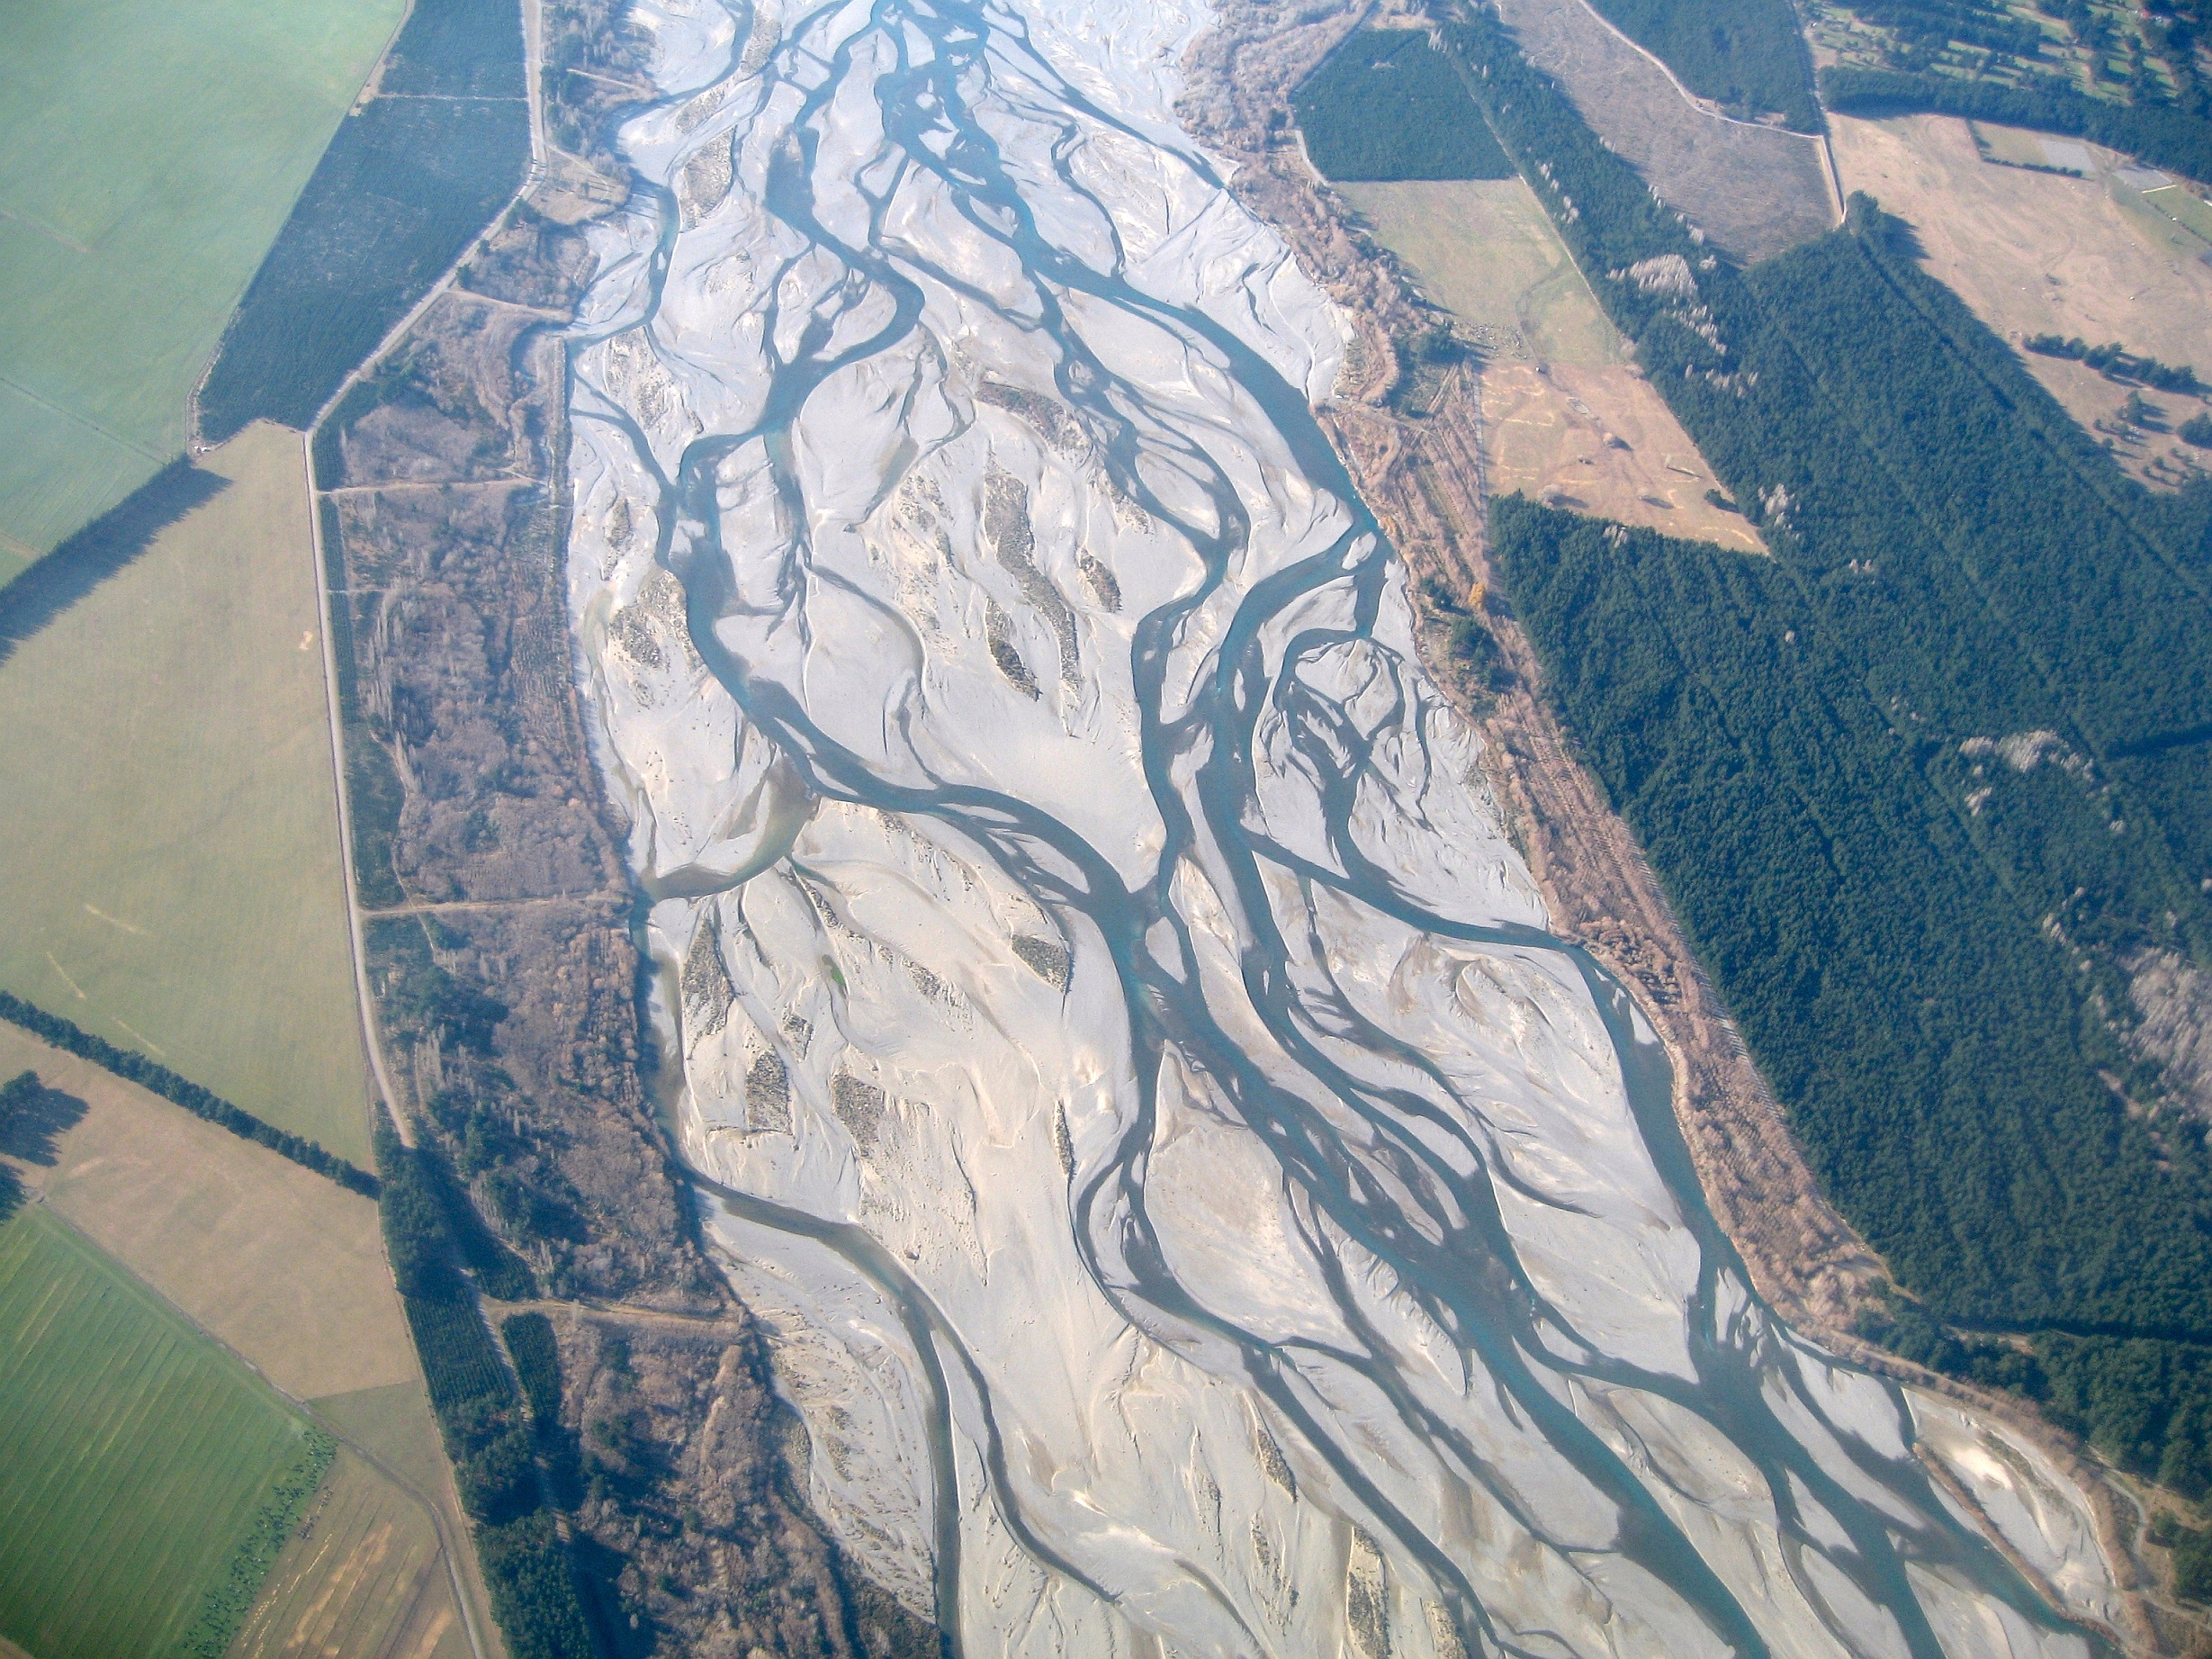
\includegraphics[width=1\linewidth]{obrazky/fluvial/divocici}
	\caption{Divočící řeka Waimakariri, Nový Zéland (Autor: Greg O'Beirne CC BY-SA 3.0)}
	\label{fig:divocici}
\end{figure}

\subsubsection{Větvící se toky}
Jedná se o přechodný typ mezi divočícím a jednoduchým (nevětvícím se) tokem. Větvící se toky mají zpravidla hlavní koryto a menší vedlejší koryta. V některých případech se jedná jen o povodňová (tzv. avulzní koryta). Štěrkové lavice větvících se toků bývají stabilnější a porostlé dřevinnou vegetací \parencite{galiaFluvialniGeomorfologie2017}.
%Při vyústění horských toků s rozkolísanými průtoky na předpolí
%Předpoklady:
%\begin{itemize}
%	\item Velké množství sedimentů
%	\item Snadno erodovatelné břehy
%	\item Velká rozkolísanost průtoků
%	\item Velký gradient údolí
%	\item Časté laterární změny v půdorysu spojené s nestabilními koryty a velkým množstvím dnových splavenin
%	\item Vznik a překládání štěrkových lavic, ostrovů atd.
%\end{itemize}

\subsection{Anastomózní toky}
Půdorysně podobné divočícímu toku jsou \emph{anastomózní toky} (\textit{anastomosed} nebo \textit{anabranching channels}). Tento typ vodního toku ale není tvořen jedním korytem členěným do celé řady větví měnících se v čase. Anastomózní tok je soustava sinusouidních až meandrujících koryt, které jsou mírně zahloubené do nivy. Vzniklé říční ostrovy jsou stabilní a porostlé vegetací. Anastomóní toky se nacházejí v nížinách.


\section{Údolí}

Tvar údolí je výsledkem vztahu mezi lineární erozí vodního toku a vývojem svahů.

\emph{Soutěsky} (hluboké soutěsky = kaňony), vznikají při převaze lineární eroze. Svahy soutěsky jsou zhruba rovnoběžné a šířka je přibližně stejná ve spodní i horní části.

\emph{Údolí ve tvaru písmene V} vznikají při rovnováze mezi zahlubováním toků a vývojem svahů. Dno údolí je tvořeno korytem vodního toku a směrem nahoru se údolí rozevírá. 

\emph{Neckovitá údolí} vznikají při převaze boční eroze vodního toku nad hloubkovou. Meandrováním vodního toku dochází k podemílání svahů tu na jedné, tu na druhé straně údolí. Vzniká údolí s širokým dnem, které je zpravidla zaplněné údolní nivou. Údolní dno přechází ostrým zálomem dno relativně příkrých svahů. 

\emph{Úvalovité údolí} je údolí se širokým dnem, které bez výrazného zálomu přechází do mírných svahů.

\begin{figure}[h]
	\centering
	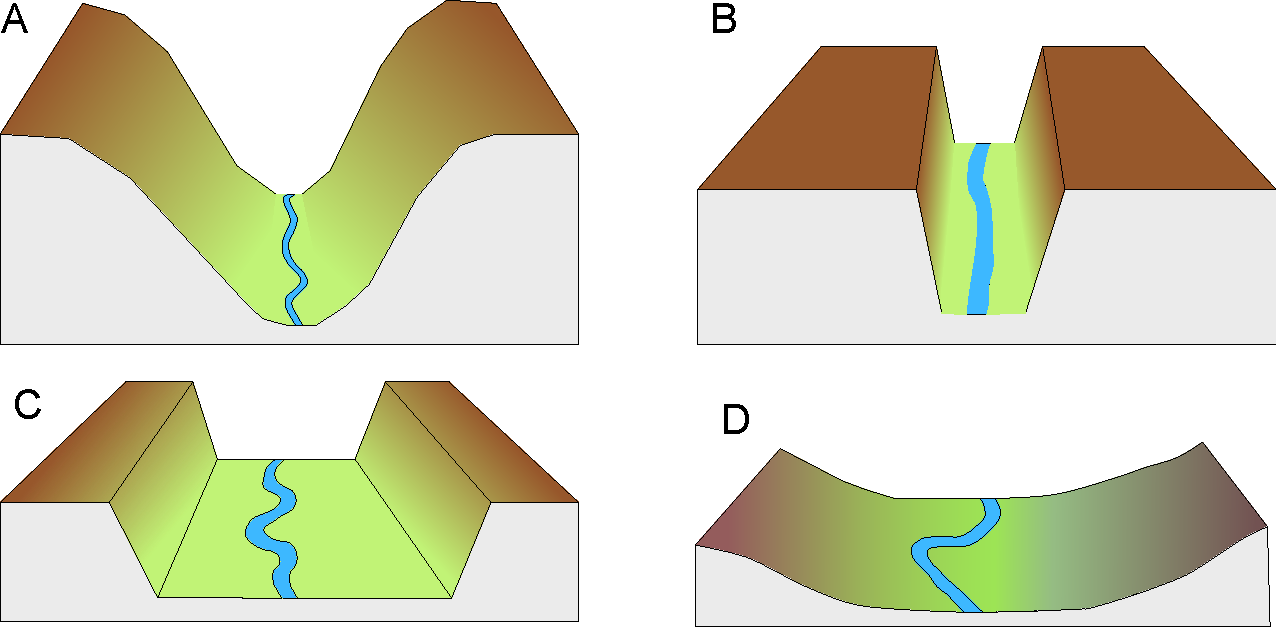
\includegraphics[width=1\linewidth]{obrazky/fluvial/typy_udoli}
	\caption{Typy údolí. A) údolí typu "V", B) soutěska, C) neckovité údolí, D) úvalovité údolí}
	\label{fig:typyudoli}
\end{figure}

\subsection{Vodní toky a morfostruktura}
Vodní toky můžeme rozdělit podle jejich vztahu k morfostruktuře. \textcite{demekObecnaGeomorfologie1987} rozlišuje \emph{konsekventní toky}, které mají směr toku určený původním sklonem georeliéfu. Tento typ vodních toků zpravidla není závislý na morfostruktuře. \emph{Subsekventní toky} jsou vázané na méně odolné horniny nebo na tektonické linie. Jejich směr je shodný se směrem a úklonem vrstev nebo shodný s průběhem tektonických linií. \emph{Resekventní toky} mají stejný směr jako konsekventní. Nacházejí se ale na erozním případně strukturním povrchu nižší úrovně než konsekventní toky. \emph{Obsekventní toky} mají směro opačný než je generelní sklon povrchu krajiny. Tento typ toků je často vázán na tektonické linie. \emph{Insekventní toky} nejsou nijak závislé na morfostruktuře či původním sklonu.

Rozlišují se i specifická průlomová údolí. \emph{Antecedentní údolí} vzniká tehdy, když se vodní tok zařezává do postupně se vyzdvihujícího se území. Je ale potřeba, aby výzdvih byl celkově pomalejší, než hloubková eroze toku. \emph{Epigenetické údolí} vzniká zařezáváním do měkkého podloží, kde i po dosažení odolnějších hornin dojde k zachování směru toku. 


\subsection{Podélný profil a erozní báze}
Podélný profil (\textit{longitudal profile}) vodního toku (také spádová křivka vodního toku) zobrazuje jak se mění nadmořská výška toku se vzdáleností od pramene k ústí. Ideální tzv. \emph{vyrovnaný podélný profil} je konkávní a hladký (bez různých zálomů). V horní části vodního toku je křivka nejstrmější a směrem k ústí se zmírňuje. Tento \enquote{ideální} vodní tok neeroduje své podloží ani neakumuluje sedimenty. Je totiž schopen veškerý materiál, který se do něj dostane např. svahovými procesy, transportovat. K vyrovnanému podélnému profilu spějí veškeré vodní toky. Je však nedostižným ideálem, protože do vývoje podélného profilu zasahuje celá řada faktorů jako je odolnost hornin, donáška sedimentů, tektonické pohyby, změny v průtoku apod. 

S podélným profilem vodního toku je třeba zmínit i \emph{erozní bázi}. Erozní báze je místo o určité nadmořské výšce pod kterou se vodní tok nedokáže zahlubovat případně se zahlubuje jen velice obtížně. \emph{Globální erozní bází} je hladina světového oceánu. \emph{Lokální erozní bází} může být ústí vodního toku do větší řeky, jezera. Může to být ale vrstva odolných hornin nebo antropogenní prvek v korytě jako je jez.




%\todo[inline]{podélný profil, erozní báze}
%\todo[inline]{vztah ke struktuře}

\section{Korytové formy}
Sedimenty unášené vodním tokem vytvářejí celou řadu různých více či méně trvanlivých forem. Při rovnováze mezi donáškou sedimentů a transportní kapacitou toku vzniká na dně štěrkonosných toků vrstva tvořená z hrubšího materiálu, než je pod povrchem. Dochází i k \emph{imbrikaci}, což je uspořádání klastů (štěrků, valounů) tak, aby jejich nejdelší osa byla kolmá na směr proudění a nejkratší osa kolmá na dno toku. Imbrikované klasty jsou odolnější vůči erozi - vzniká \emph{armovaná vrstva}.

Typickým tvarem vodních toků s písečným dnem jsou \emph{čeřiny a duny} (\textit{dunes, ripples}). Jedná se o mobilní korytové formace. Čeřiny vznikají již při velice nízkých rychlostech proudění. Duny vznikají při vyšších rychlostech. 

Z větších klastů jsou tvořené \emph{sedimentární klastry} (\textit{particle clusters}). Jedná se o shluky štěrků či valounů, uložených nad a pod základním (největším) valounem (Obr. \ref{fig:klastklastr}). 

\begin{figure}
	\centering
	\includegraphics[width=1\linewidth]{obrazky/fluvial/klast_klastr}
	\caption{Znázornění sedimentárního klastru. Upraveno podle \textcite{galiaFluvialniGeomorfologie2017})}
	\label{fig:klastklastr}
\end{figure}

Běžným tvarem, který nacházíme v korytě jsou \emph{štěrkové a písčité lavice} (Obr. \ref{fig:lavice}). Jedná se o nánosy štěrku (písku). Vznikají v rozličných pozicích a z různých příčin. Obecně se dá ale říct, že hlavním důvodem jejich vzniku je ztráta unášecí schopnosti toku. \emph{Střídavé lavice} se nacházejí (\textit{alternat bars}) střídavě u jednoho a u druhého břehu. Vznikají během sestupné fáze povodňové vlny (při klesajícím vodním stavu). Střídavé lavice způsobují rozkmitání proudnice. Na soutocích můžeme spatřit \emph{soutokové lavice} (\textit{channle junction bars}). \emph{Diagonální lavice} (\textit{diagonal bars}) procházejí šikmo korytem. Vznikají v místech rozšíření koryta, kde vodní tok ztrácí energii nebo je v daném místě větší donáška sedimentů. \emph{Středové lavice} (\textit{mid-channel bars}) mohou vznikat z diagonálních. Nacházíme je v divočících tocích. \emph{Vrcholové lavice} (\textit{point bars}) se nacházejí na vnitřní (akumulační) straně meandru jako důsledek pomalejšího proudění a působení sekundárních proudů.

\begin{figure}
	\centering
	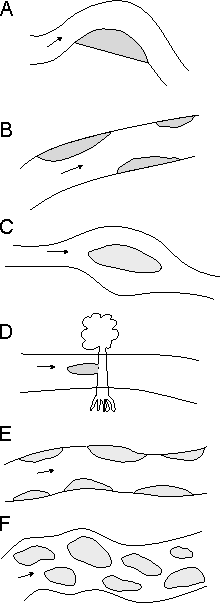
\includegraphics[width=1\linewidth]{obrazky/fluvial/lavice}
	\caption{Příklad některých lavic, které lze nalézt v říčním korytě. A vrcholové lavice, B střídavé lavice, C středové lavice (bermy), D lavice před překážkou, E nepravidelné lavice, F lavice v divočícím toku  (upraveno podle \textcite{radecki-pawlikStreamHydraulicsGranulometry2004} }
	\label{fig:lavice}
\end{figure}

\section{Mimokorytové formy}
\subsection{Niva}
\emph{Niva} (\textit{floodplain}) je akumulační plošina v okolí vodního toku, která je pravidelně zaplavována. Nivu najdeme v okolí většiny řek. Výjimku tvoří toky v horském prostředí, které mají vysokou transportní kapacitu, a kde v sevřených údolích není prostor pro její vývoj. Šířka nivy se zpravidla odvíjí od velikosti řeky, jejího průtoku. Mohutnější řeka bude mít širší nivu, než její menší přítoky. 

Ukládání sedimentů v nivě probíhá vertikální a boční akrecí. K \emph{vertikální akreci} dochází při rozlití vody do nivy při povodňové události. Voda v důsledku větší drsnosti nivy proudí pomaleji, což snižuje její schopnost transportovat sedimenty a ty se ukládají na povrch nivy. Jejich množství a zrnitost klesá směrem od koryta. Důsledkem této nerovnoměrné distribuce sedimentů v nivě je vznik \emph{agradačních (břehových) valů} (\textit{levees}) kolem koryta. Jsou tvořeny hlavně písčitými sedimenty a mohou mít výšku v řádu decimetrů až několika metrů. Ve větší vzdálenosti od koryta se ukládá jemnozrnnější materiál (prach, jíl), což označujeme jako facii \emph{povodňových hlín}. \emph{Boční (laterální) akrece} je výsledkem migrace toku do stran. Typické je posouvání meandrů, kdy na vnitřní straně dochází k ukládání vrcholové štěrkové lavice. Ta tvoří tzv. \emph{korytovou facii}. Protrhnutím meandrové šíje vznikají slepá a mrtvá ramena. Ty mají specifické sedimenty s velkým obsahem organické hmoty -- \emph{facie opuštěných koryt}.

%\todo[inline]{obrázek nivy akrece}

\begin{figure}[h]
	\centering
	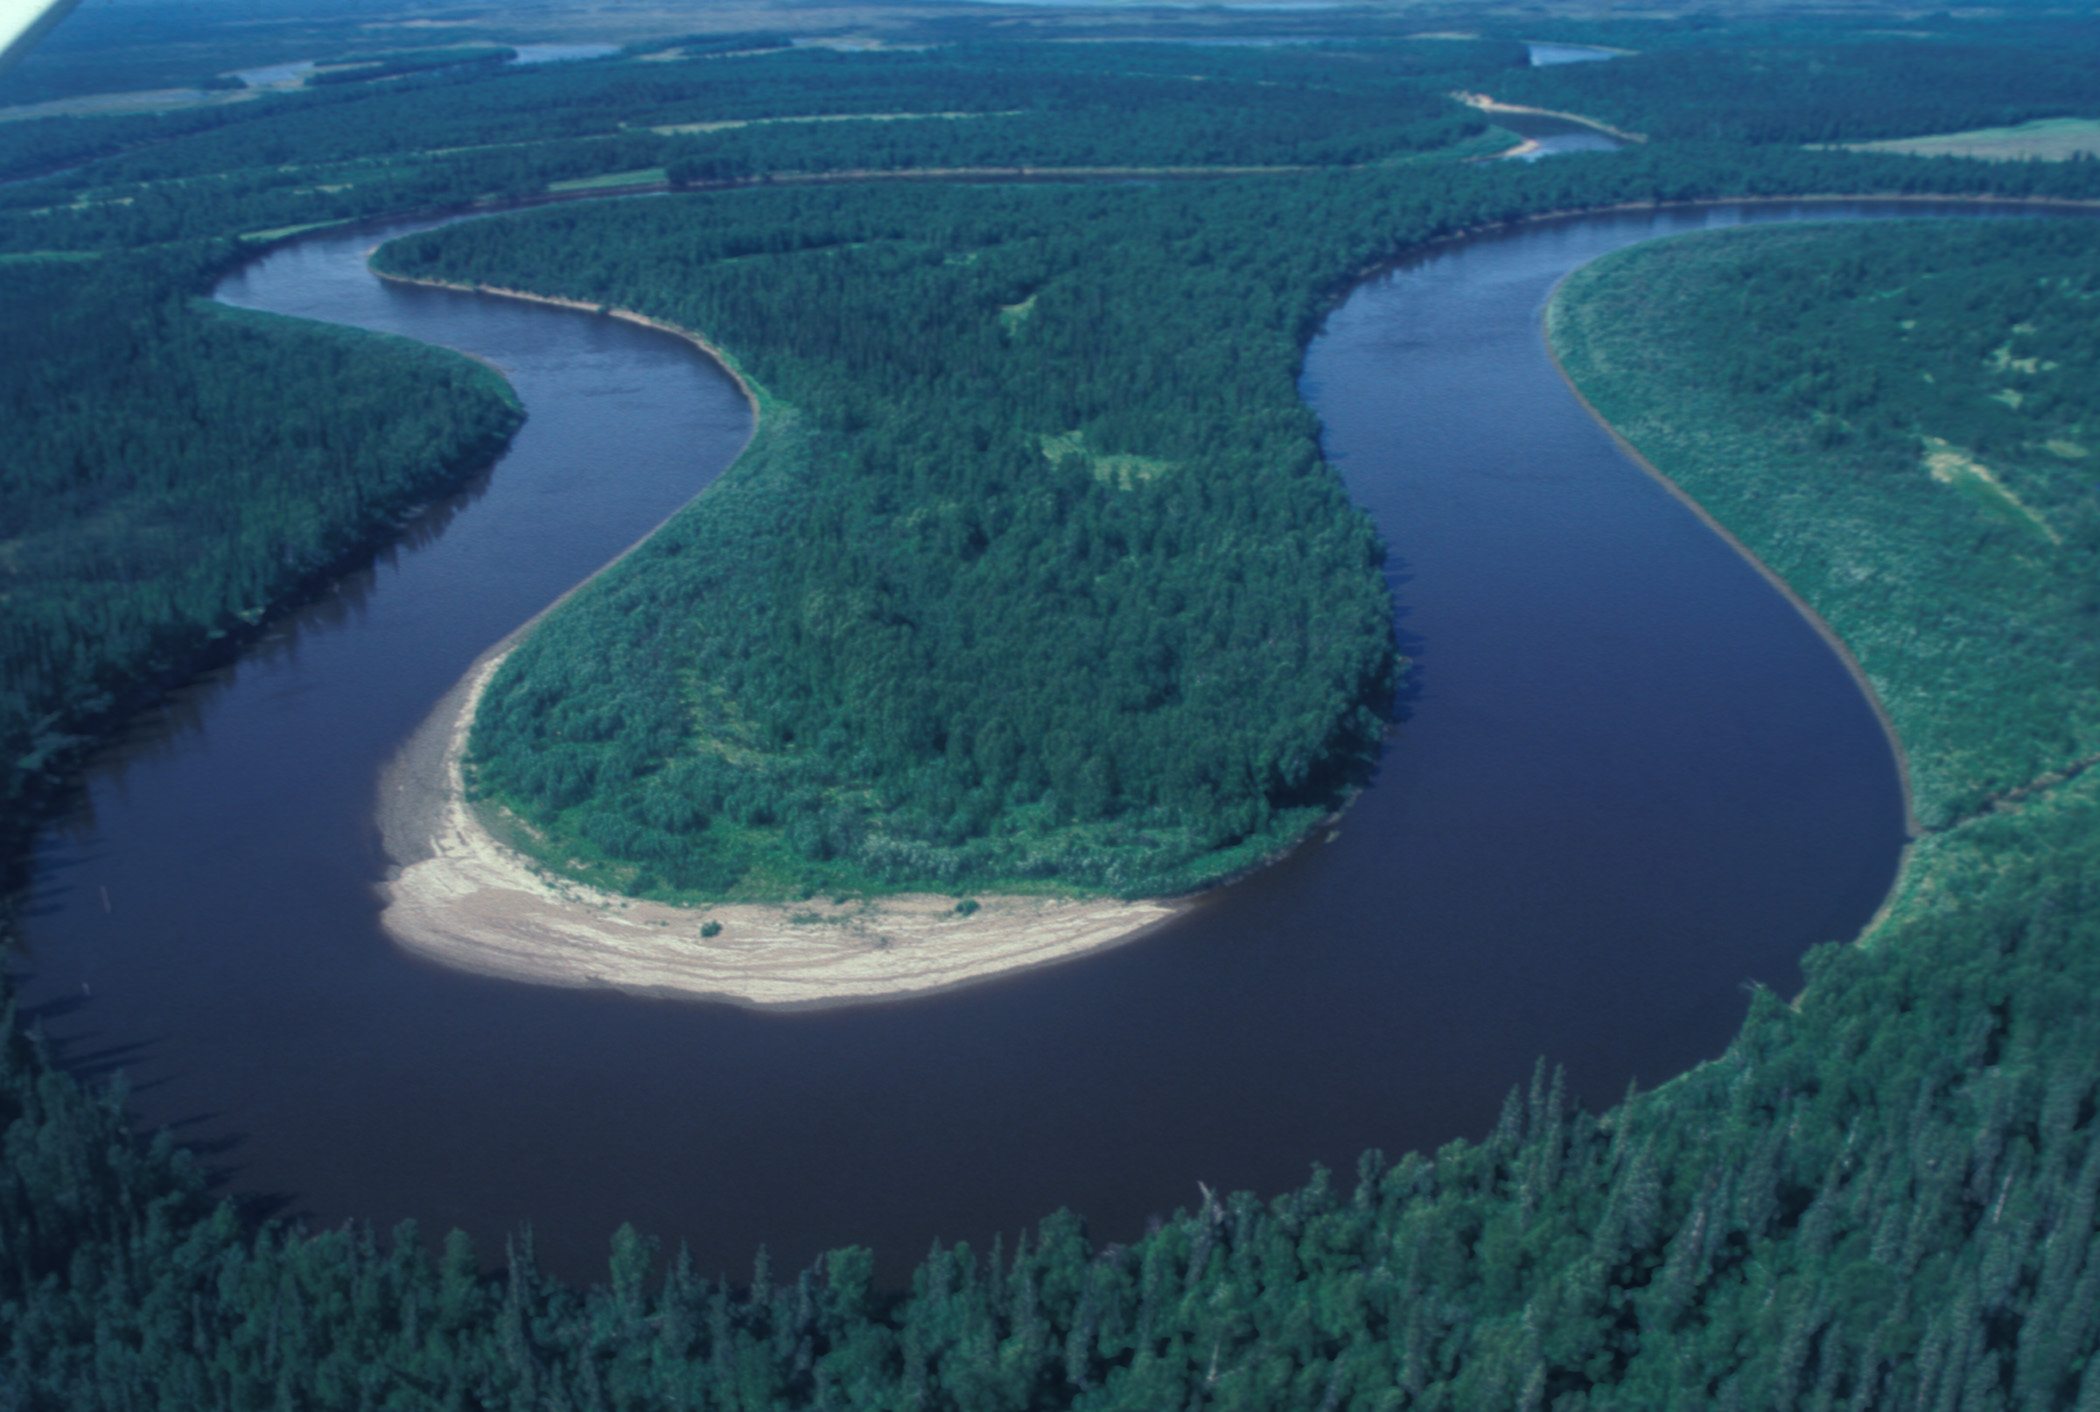
\includegraphics[width=1\linewidth]{obrazky/fluvial/meander}
	\caption{Meandrující řeka. (USGS, volné dílo)}
	\label{fig:meander}
\end{figure}

\subsection{Říční terasy}
\emph{Říční terasy} (\textit{river terraces}) jsou zbytky údolních den, které se nacházejí v různých výškách nad současným vodním tokem. Vznikly v důsledku zahloubení toku. Říční terasa se skládá z plošiny terasy a terasového stupně. \emph{Plošina terasy} je zbytek povrchu staré nivy. \emph{Terasový stupeň (svah)} odděluje terasu od současné nivy nebo terasy jiné úrovně. Terasy dělíme na skalní terasy (strath) a aluviální terasy. \emph{Skalní (strath) terasy} mají jen tenkou pokrývku ze sedimentů a jsou erozního původu. Terasy v aluviu mohou být akumulační a erozní. \emph{Akumulační terasy} jsou zbytky údolní nivy, které vodní tok prořízly až na skalní podklad. Pokud se vodní tok neproeroduje až na skalní podloži, vznikají \emph{vložené erozní terasy}. Dále se terasy dělí na \emph{párové} (vyskytují se na obou stranách údolí) a \emph{nepárové} (je pouze na jedné straně údolí). Vznik teras je ovlivněn změnami klimatu, oscilací erozních bází nebo tektonickou aktivitou. 
%\todo{doplnit terasy} 

\subsection{Náplavový kužel}
\emph{Náplavový kužel} (\textit{alluvial fan}) je akumulační forma ve formě vějíře či kuželu. Vrchol kužele je v místě vyústění vodního toku z horského terénu do podhůří nebo mezihorských pánví. Velká změna sklonu a rozevření údolí způsobuje, že vodní tok ztrácí schopnost unášet sedimenty a ty se začínají akumulovat. 

\begin{figure}[h]
	\centering
	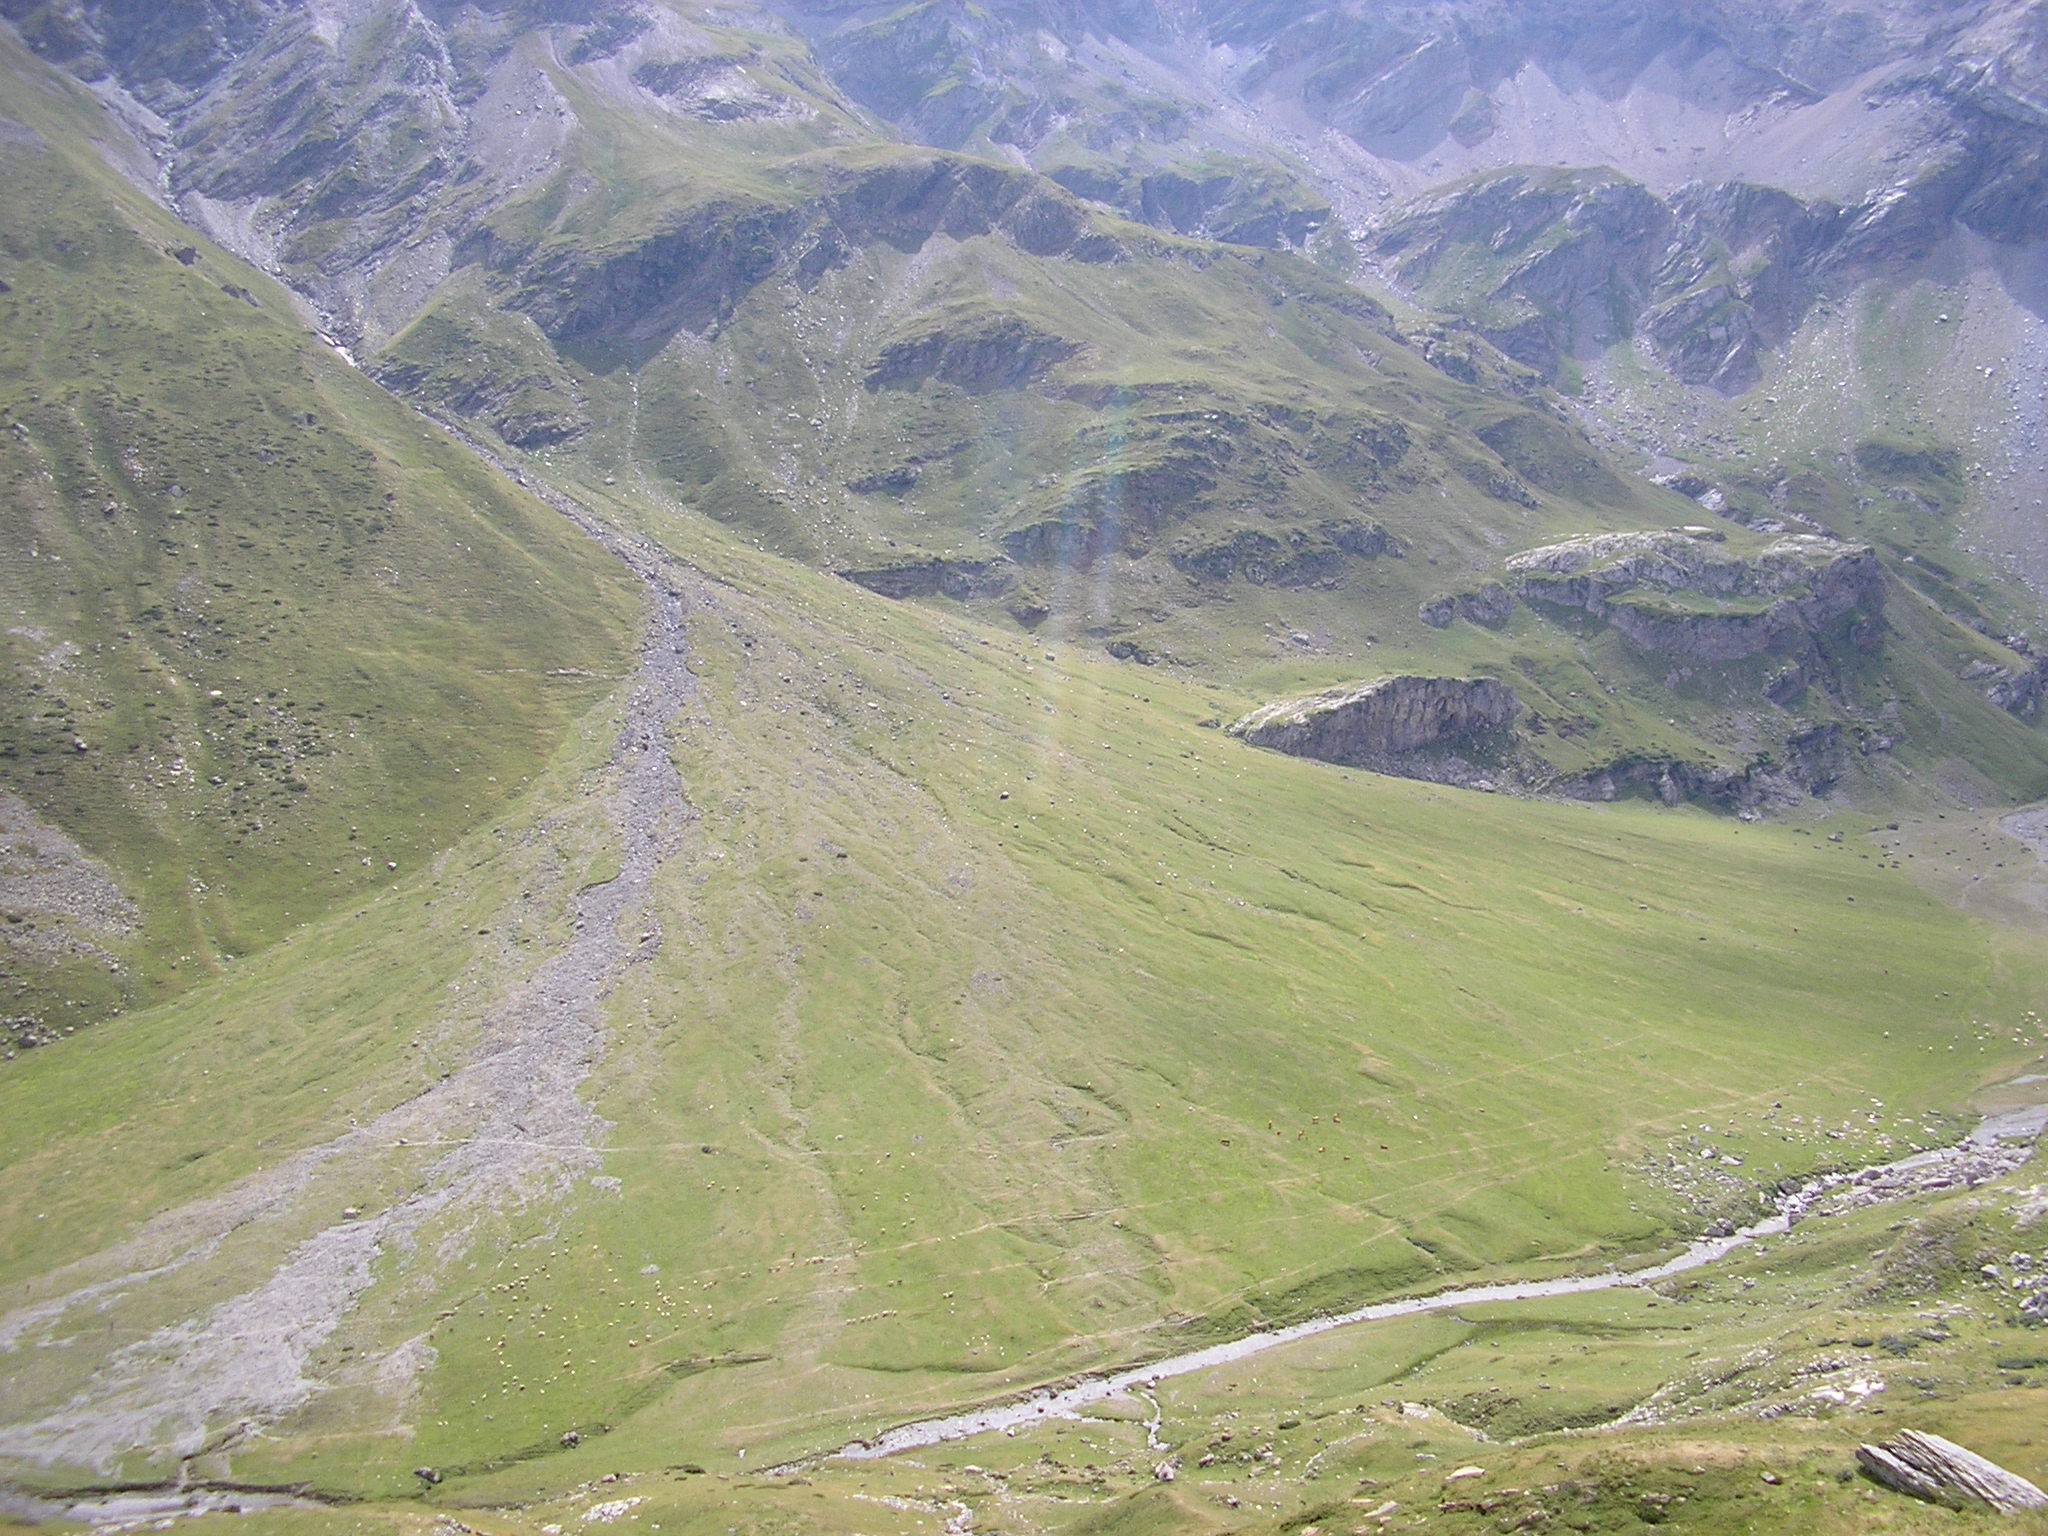
\includegraphics[width=1\linewidth]{obrazky/fluvial/Alluvial_fan}
	\caption{Menší aluviální kužel v Pyrenejích (Autor: Mikenorton, CC BY-SA 3.0 via Wikimedia Commons)}
	\label{fig:alluvialfan}
\end{figure}

Vodní tok se na náplavovém kuželu různě větví. U velkého množství náplavových kuželů dochází k zařezávání toku v jeho horní části. To způsobuje posouvání akumulace do distálních (koncových) poloh kužele. 

Fluviální sedimenty jsou na kuželu tříděné, jelikož vodní tok postupně ztrácí unášecí schopnost. V horní části kuželu jsou větší klasty a směrem k jeho spodní části se zjemňují. Na vzniku kuželů se mohou podílet i blokovobahenní proudy (viz \ref{blokovo}), jejichž sediment nemá takový stupeň vytřízení jako materiál transportován řekou. Kužely, tvořené kombinací sedimentů blokovobahenních proudů a aluviálních, označujeme jako \emph{proluviální kužely}.

Spojením velkých kuželů na úpatí pohoří do jednoho rozsáhlého celku vzniká \emph{bahadový reliéf} (\textit{bajada}). 

\begin{figure}[h]
	\centering
	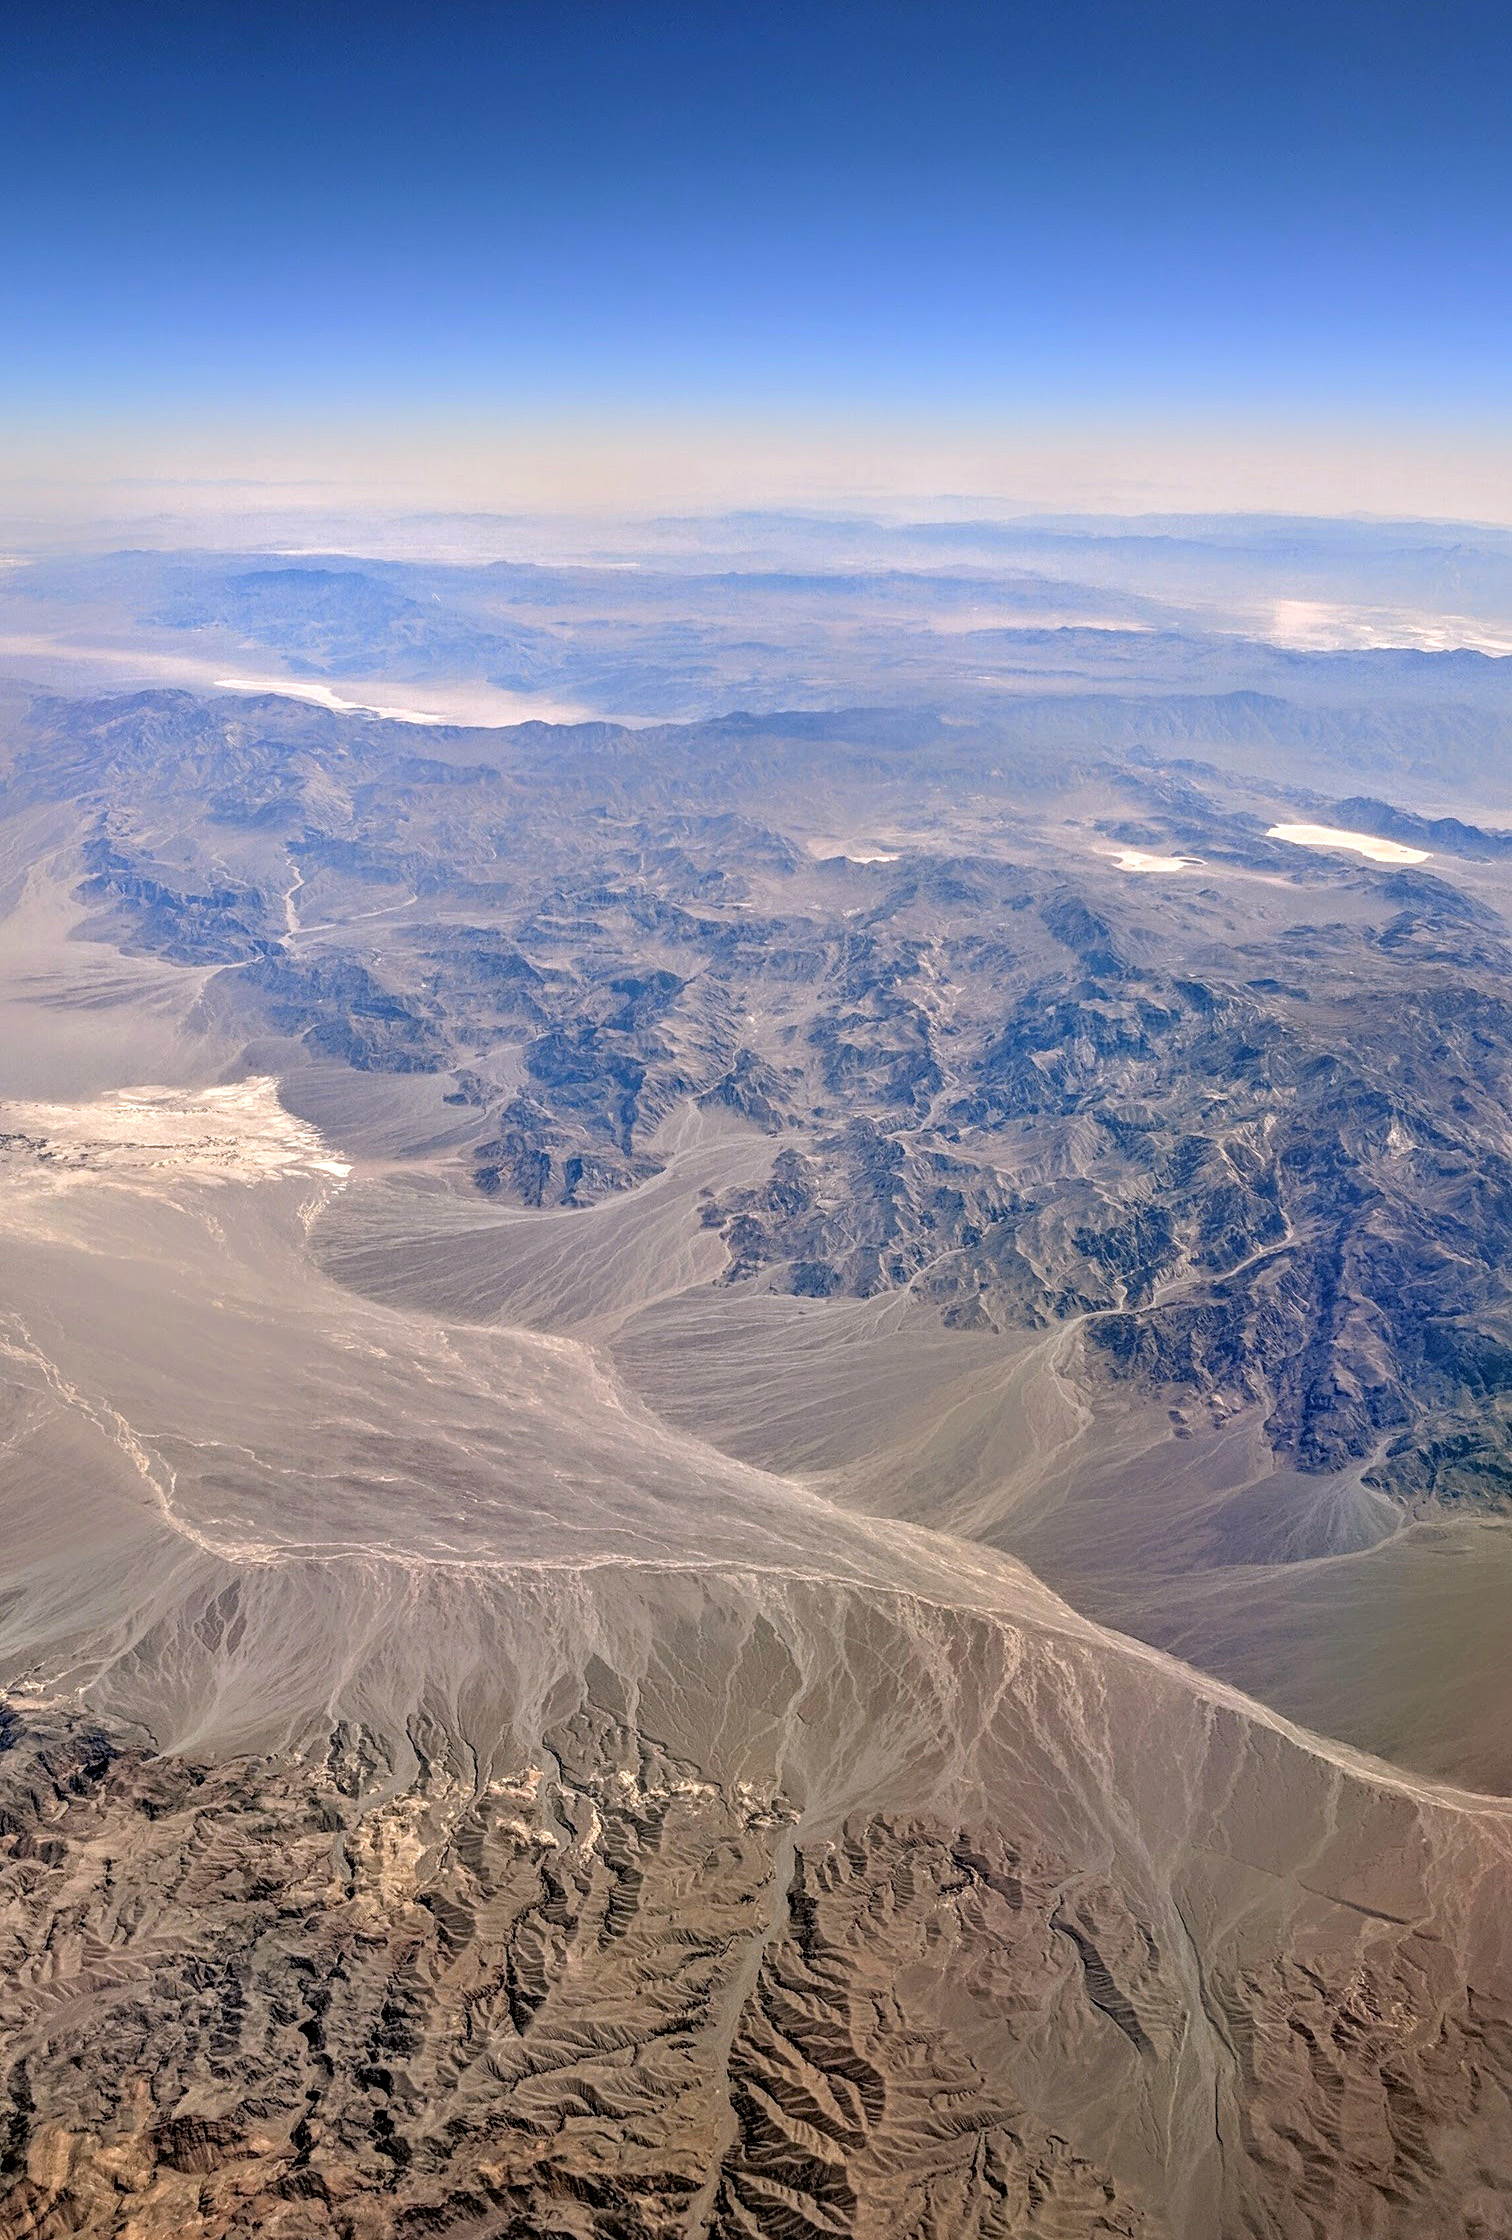
\includegraphics[width=1\linewidth]{obrazky/fluvial/bajada}
	\caption{Bajady v Údolí smrti (Autor: Dicklyon, CC BY-SA 4.0 via Wikimedia Commons)}
	\label{fig:bajada}
\end{figure}

\newpage
\onecolumn
\begin{boxotazky}{Kontrolní a klíčové otázky, na které bychom měli znát odpověď}
	\begin{itemize}
		\item 
		\item 
		
	\end{itemize}
\end{boxotazky}

\begin{boxslovnik}{Další klíčové pojmy k zapamatování}
	aaa & adfasd \\
	
\end{boxslovnik}
\twocolumn